\documentclass{article}

\usepackage[tmargin=1in,bmargin=1in,lmargin=1.25in,rmargin=1.25in]{geometry}
\usepackage{graphicx}
\usepackage{hyperref}
\usepackage{amsmath}
\usepackage{subcaption} % subfigures
%\usepackage{matlab}

\thispagestyle{empty}

\begin{document}


\title{ \normalsize \textsc{}
	\\ [2.0cm]
%	\HRule{1.5pt} \\
	\Large \textbf{\uppercase{Optimizing a High-Dimension Compartment ODE Model}
}
}
\date{December 2023}
\author{Jeremy Chiu,\\APMA 923, Dr. JF Williams} 
	

\maketitle
%\newpage
%\tableofcontents

\section{Project Overview}

We consider the compartment ODE model presented by Guo-Wu\cite{GuoWu}, which describes the spread of Tuberculosis (TB) among the Canadian foreign-born population.  Their ODE model features 5 dependent variables (each requiring an initial condition) and 9 parameters, some of which are physically difficult to measure or estimate.  Our goal is to find the combination of parameters and initial conditions that give the global minimum of the model's prediction error, which is defined by comparing model output to reported TB incidence data.

\subsection{Background and loss function}


We consider the compartment ODE model presented by Guo-Wu\cite{GuoWu}, which describes the spread of Tuberculosis (TB) among the Canadian foreign-born population.  Fundamentally, an SEIR-model is used, where the \textit{exposed} category is partitioned into \textit{early latent} and \textit{late latent}.  Figure \ref{fig:flow} shows an overview of their model.

\begin{figure}
	\centering 
		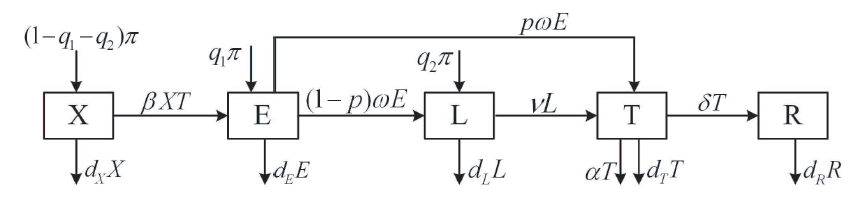
\includegraphics[scale=0.4]{xeltr flow diagram}
		\caption{Flow diagram of the compartment ODE model used by \cite{GuoWu}.}
		\label{fig:flow}
\end{figure}

After fixing initial conditions and parameter values, we use Matlab's \texttt{ode23} routine to solve the system of differential equations from \cite{GuoWu}, which returns population vs time.  From the population, we compute the TB incidence
$$\text{Estimated TB Incidence } = \frac{100,000}{X(t)+E(t)+L(t)+T(t)+R(t)} \cdot (pw E(t) + v L(t)) ,$$
which can be compared to the reported TB incidence from Canadian reports\cite{MounchiliA.2022TuberculosisReport} (see figure \ref{fig:foreignBornData}).  We use data from 2010-2020.  The error is defined to be the difference between our computed (estimated) incidence and the reported incidence.  We use parameters that are difficult to measure as input to the optimizer: $q_1$ and $q_2$ are the percentage of new immigrants that are undetected by Canadian TB screening, and the initial populations $E_0$, $L_0$, and $R_0$ are unknown; for a total of 5 variables to optimize across.  Note that $T_0$ is reported, and $X_0$ is computed from the reported total foreign-born population.  All other parameters use estimates found from the medical and epidemiological literature.

\begin{figure}
	\centering 
	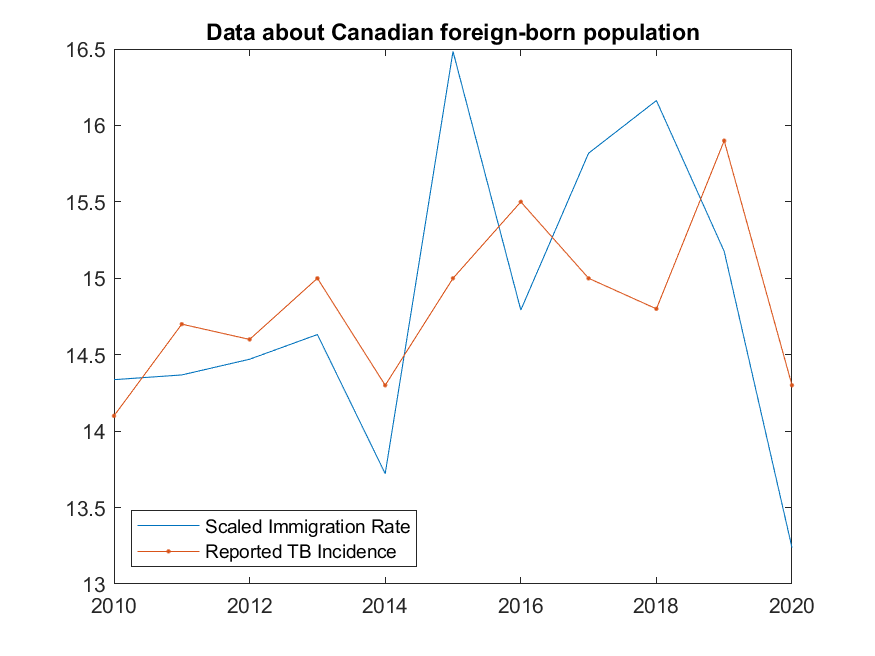
\includegraphics[scale=0.6]{foreignBornData}
	\caption{Reported incidence of Canadian foreign-born population.  Annual immigration rate is also presented, scaled to be on same viewing rectangle.  Notice how the number of immigrants drive the incidence rate.}
	\label{fig:foreignBornData}
\end{figure}


	\subsection{Project Proposal Meeting}
	
	JF and I met on October 27 to discuss the project.  Here were JF's suggestions about possible things to try:
	
	\begin{itemize}
		\item Do not over expand on problem background.  Discuss how we solved it.
		\item Compare solvers.
		\item Try to find local sensitivity.  Investigate derivatives with respect to parameters.
		\item Discuss \texttt{fmincon}.
		\item Global optimization toolbox.
		\item Find an upper bound on $q_1$ and $q_2$ using immigration data.
		\item Investigate convexity.
	\end{itemize}

	\section{Finding the global min with \texttt{fmincon}}

	We used Matlab's constrained solver, \texttt{fmincon}.  Our constraints were 
	$$ q_1,~q_2,~E_0,~L_0,~R_0 \geq 0, \text{ and } q_1+q_2 \leq 1$$
	Initial conditions were the original proportions presented in \cite{GuoWu}.  The solver does a decent job in minimization -- figure \ref{fig:optimizedIncidence} shows the estimated incidence after optimization, which is reasonably close to the reported incidence.
	
	\begin{figure}
		\centering 
		\includegraphics[scale=0.6]{{PopVsTime_optimized}}
		\caption{After optimization, the model reasonably estimate incidence.}
		\label{fig:optimizedIncidence}
	\end{figure}
	
	\subsection{Sensitivity analysis}
	
	Aside from the 5 variables we optimized across, we had various parameters that we fixed from the literature review.  We explored the impact these parameters had on our model by simulating over a range of their values.  In total, over 2000 combinations were tried, and so the simulations must be carefully stored and interpreted.
	
	As demonstrated in figure \ref{fig:SensitivtyBigPlot}, we found that the results are most sensitive to $\nu$, $\omega$, and $L_0$; this may be unsurprising since they explicitly appear in the loss function.  However, although $E_0$ appears in the loss function, our model is not sensitive to its choice. 
	
	
	\begin{figure}
		\centering
		\begin{subfigure}[b]{0.475\textwidth}
			\centering
			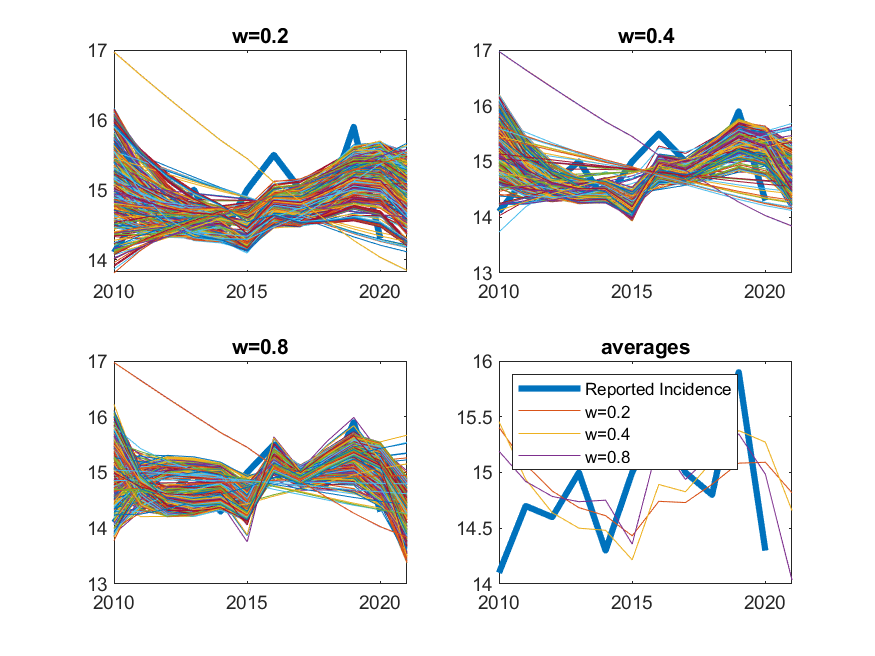
\includegraphics[width=\textwidth]{Sensitivty_w Run 2.png}
		\end{subfigure} 
		\hfill   
		\begin{subfigure}[b]{0.475\textwidth}
			\centering
			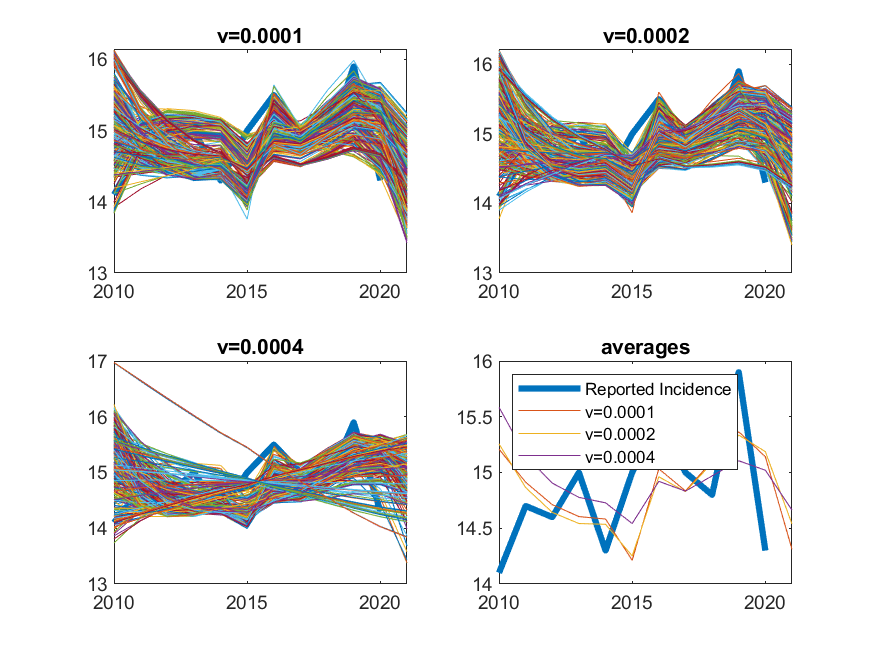
\includegraphics[width=\textwidth]{Sensitivty_v Run 2.png}  
		\end{subfigure} 
		\vskip\baselineskip
		
		\begin{subfigure}[b]{0.475\textwidth}
			\centering
			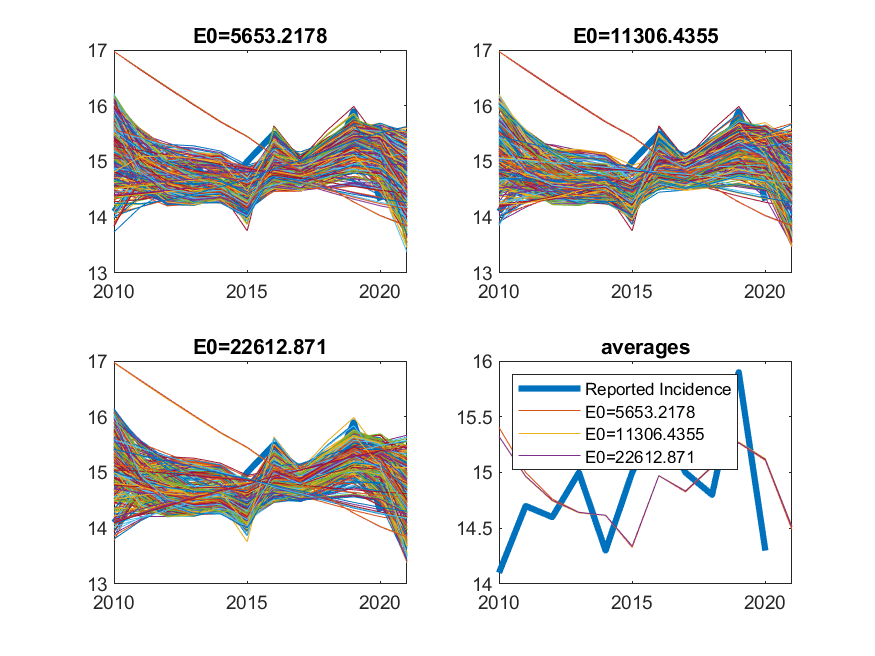
\includegraphics[width=\textwidth]{Sensitivty_E0 Run 2.png}  
		\end{subfigure} 
		\hfill
		\begin{subfigure}[b]{0.475\textwidth}
			\centering
			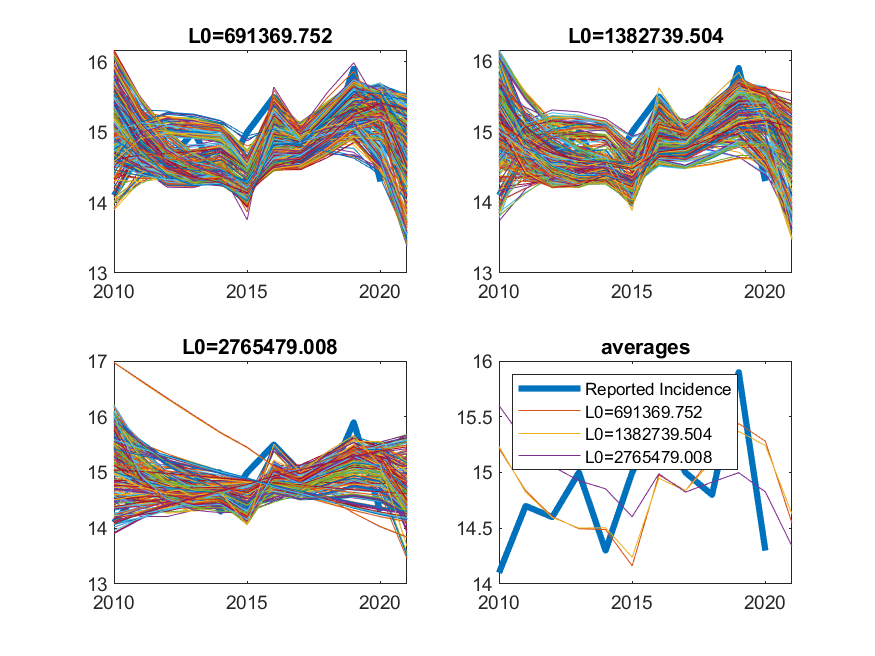
\includegraphics[width=\textwidth]{Sensitivty_L0 Run 2.png}  
		\end{subfigure} 
		
		\caption{Our results were most sensitive across $\nu$, $\omega$, and $\L_0$. There is little sensitivity across the choice of initial $E_0$.}
		\label{fig:SensitivtyBigPlot}
	\end{figure}
	
	\subsubsection{Histogram and two issues}
	
	We also explored the results of the sensitivity analysis by looking at the distribution of optimized variables.  Figure \ref{fig:est_dist} (a) gives a histogram for the optimized estimates of each of $q_1$, $q_2$, $E_0$, $L_0$ and $R_0$.  The histogram demonstrates two issues:
	
	\begin{enumerate}
		\item Many optimal solutions are near $(q_1,q_2)=(0,0)$.
		\item The optimal $L_0$ and $R_0$ are often very similar to its initial choice.
	\end{enumerate}
		
Issue 1)  Figure \ref{fig:est_dist} (a) shows many optimal $q_1$ and $q_2$ are nearly 0.  $q_2=0$ is non-realistic, because it would mean there are no immigrants with latent TB, which is unlikely because latent TB cannot be detected by many TB-infectivity tests.  Moreover, some immigrants come from countries where more than half the population is infected with TB, and our screening process targets identifying people with actively infectious TB.  For now, this issue can be avoided by discarding the non-realistic solutions.  Going forward, we should be careful with how we select initial conditions that result in $(q_1,q_2)=(0,0)$.

Issue 2) is more problematic.  The optimizer is failing to look across $L_0$ and $R_0$.  The optimal solution being near the initial condition means whatever we specify as the initial condition becomes the optimal solution.  This would force us to have accurate measurements of $L_0$ and $R_0$ to gain realistic results; unfortunately, $L_0$ and $R_0$ are difficult to measure in the real-world.  Figure \ref{fig:est_dist} (b) highlights how $L_0$ and $R_0$ are very frequently near the initial condition.  We should aim to either non-dimensionalize and remove them from the optimizer, or find a way to accurately specify them.  Another way to interpret issue 2 is that our optimizer is currently sensitive to the initial condition for $L_0$ and $R_0$.






\begin{figure}
	
	\centering
	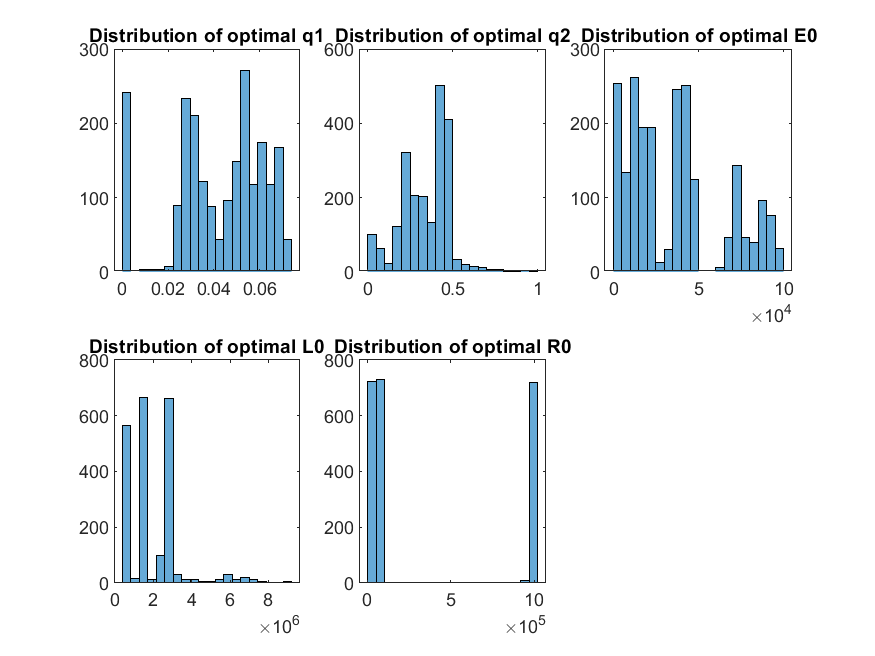
\includegraphics[width=0.45\textwidth]{Optimized parameter distribution across sensitivity analysis Run 2.png}  ~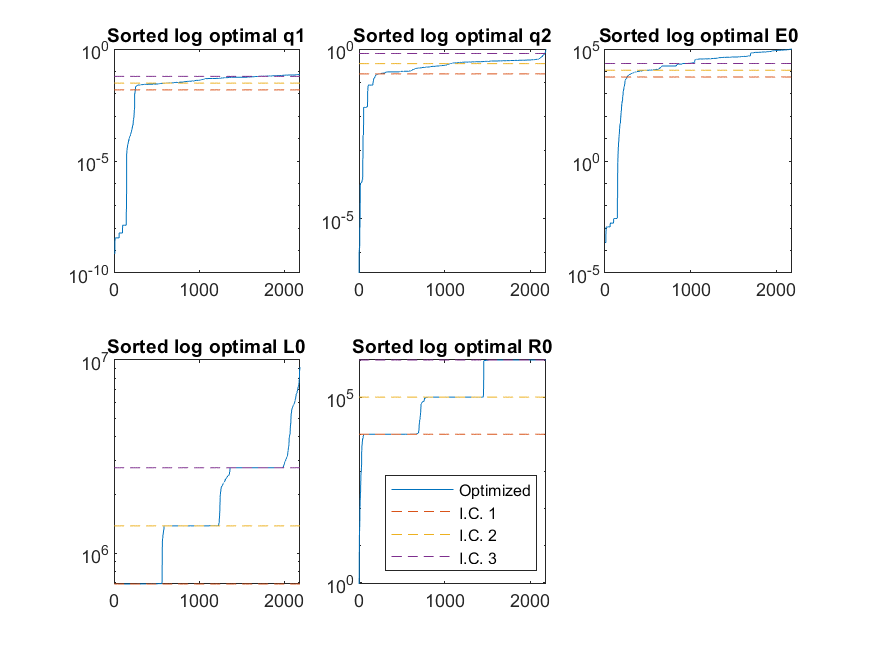
\includegraphics[width=0.45\textwidth]{Optimized parameter log sorted with starting values Run 2.png}
	
	\caption{(a) Historgram of optimized parameters.  Notice the $L_0$ and $R_0$ are similar to their initial value. (b) The optimal variables are sorted and plotted, along with the initial value.  Notice how many of the optimal $L_0$ and $R_0$ are very similar to the initial condition.  The optimal values were logged for a better viewing rectangle.}
	
	\label{fig:est_dist}
\end{figure}

\subsubsection{Distribution of error vs optimal parameter}

To get a sense of how the optimal solutions are performing, for each variable, we plot the error vs the output of the optimizer, presented in figure \ref{fig:ScatterErrorVsOptimizedParam}.  We prune outliers and continue to zoom in, but see more and more apparent outliers.  I spoke with Will Ruth (who just finished his PhD in statistics with Richard Lockhart) who commented, ``This is what the tail of a distribution will often look like. It suggests that the outliers aren't typos."  

In the scatter plot for $R_0$ in figure \ref{fig:ScatterErrorVsOptimizedParam}, notice the three vertical lines correspond to the initial conditions.

\begin{figure}
	\centering
	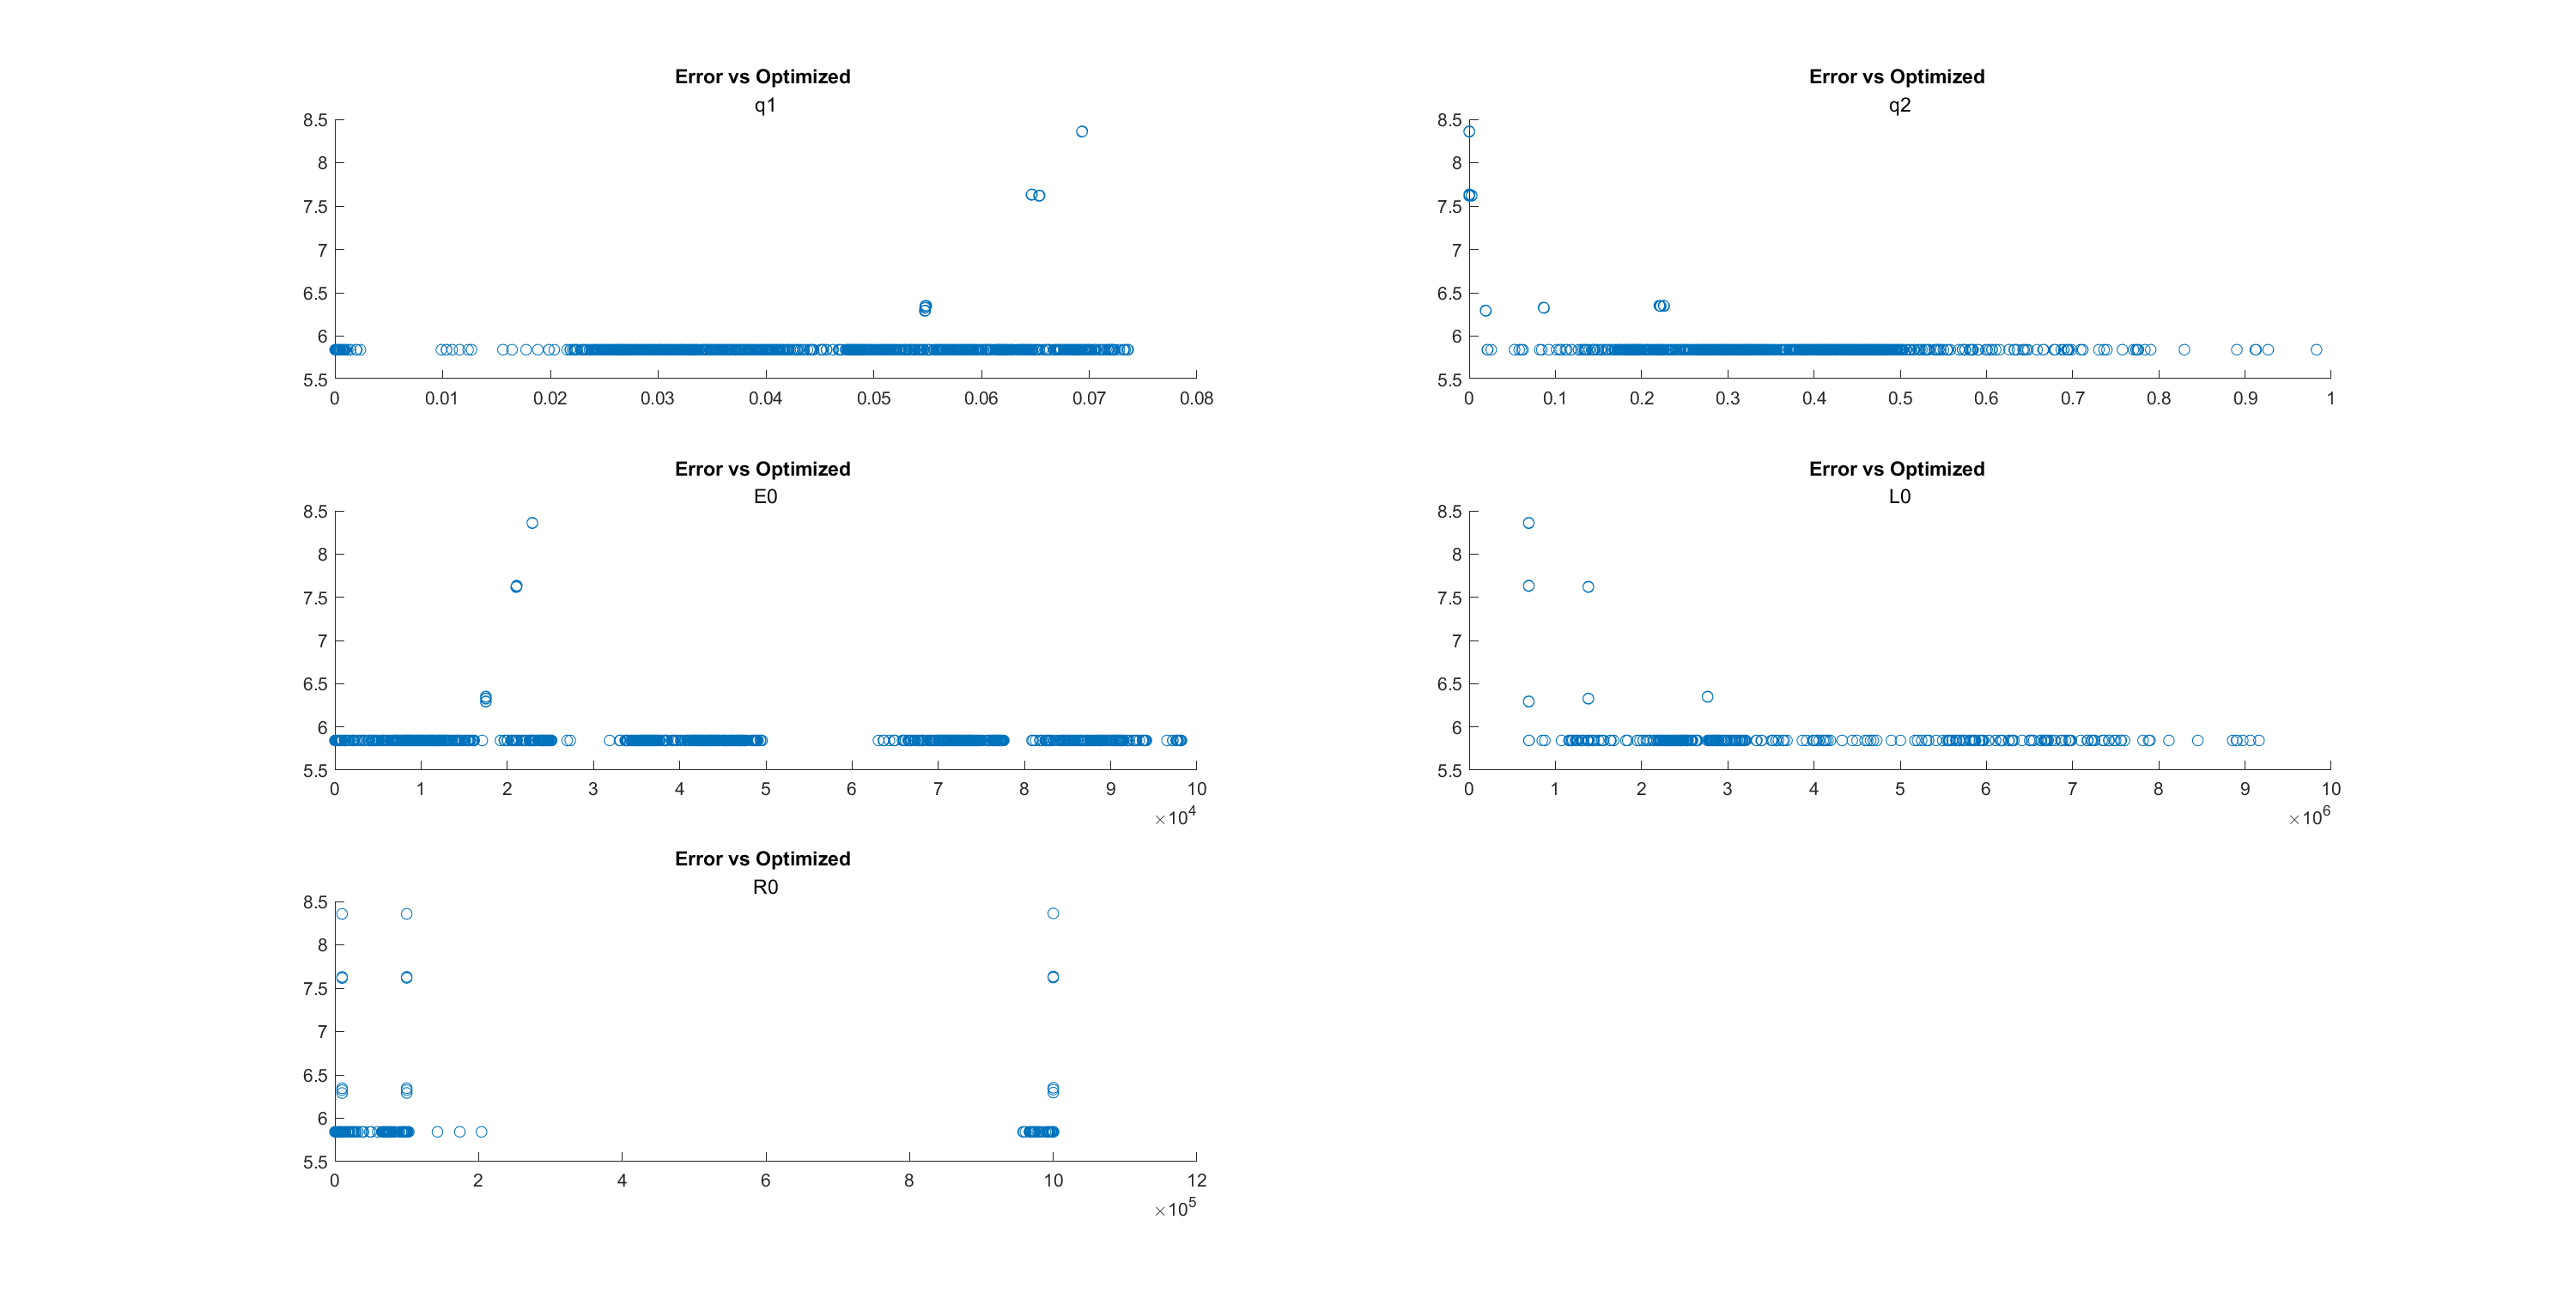
\includegraphics[width=0.8\textwidth]{ScatterPlotErrorVsOptimalOutput_Cut2.png}  
	
	
	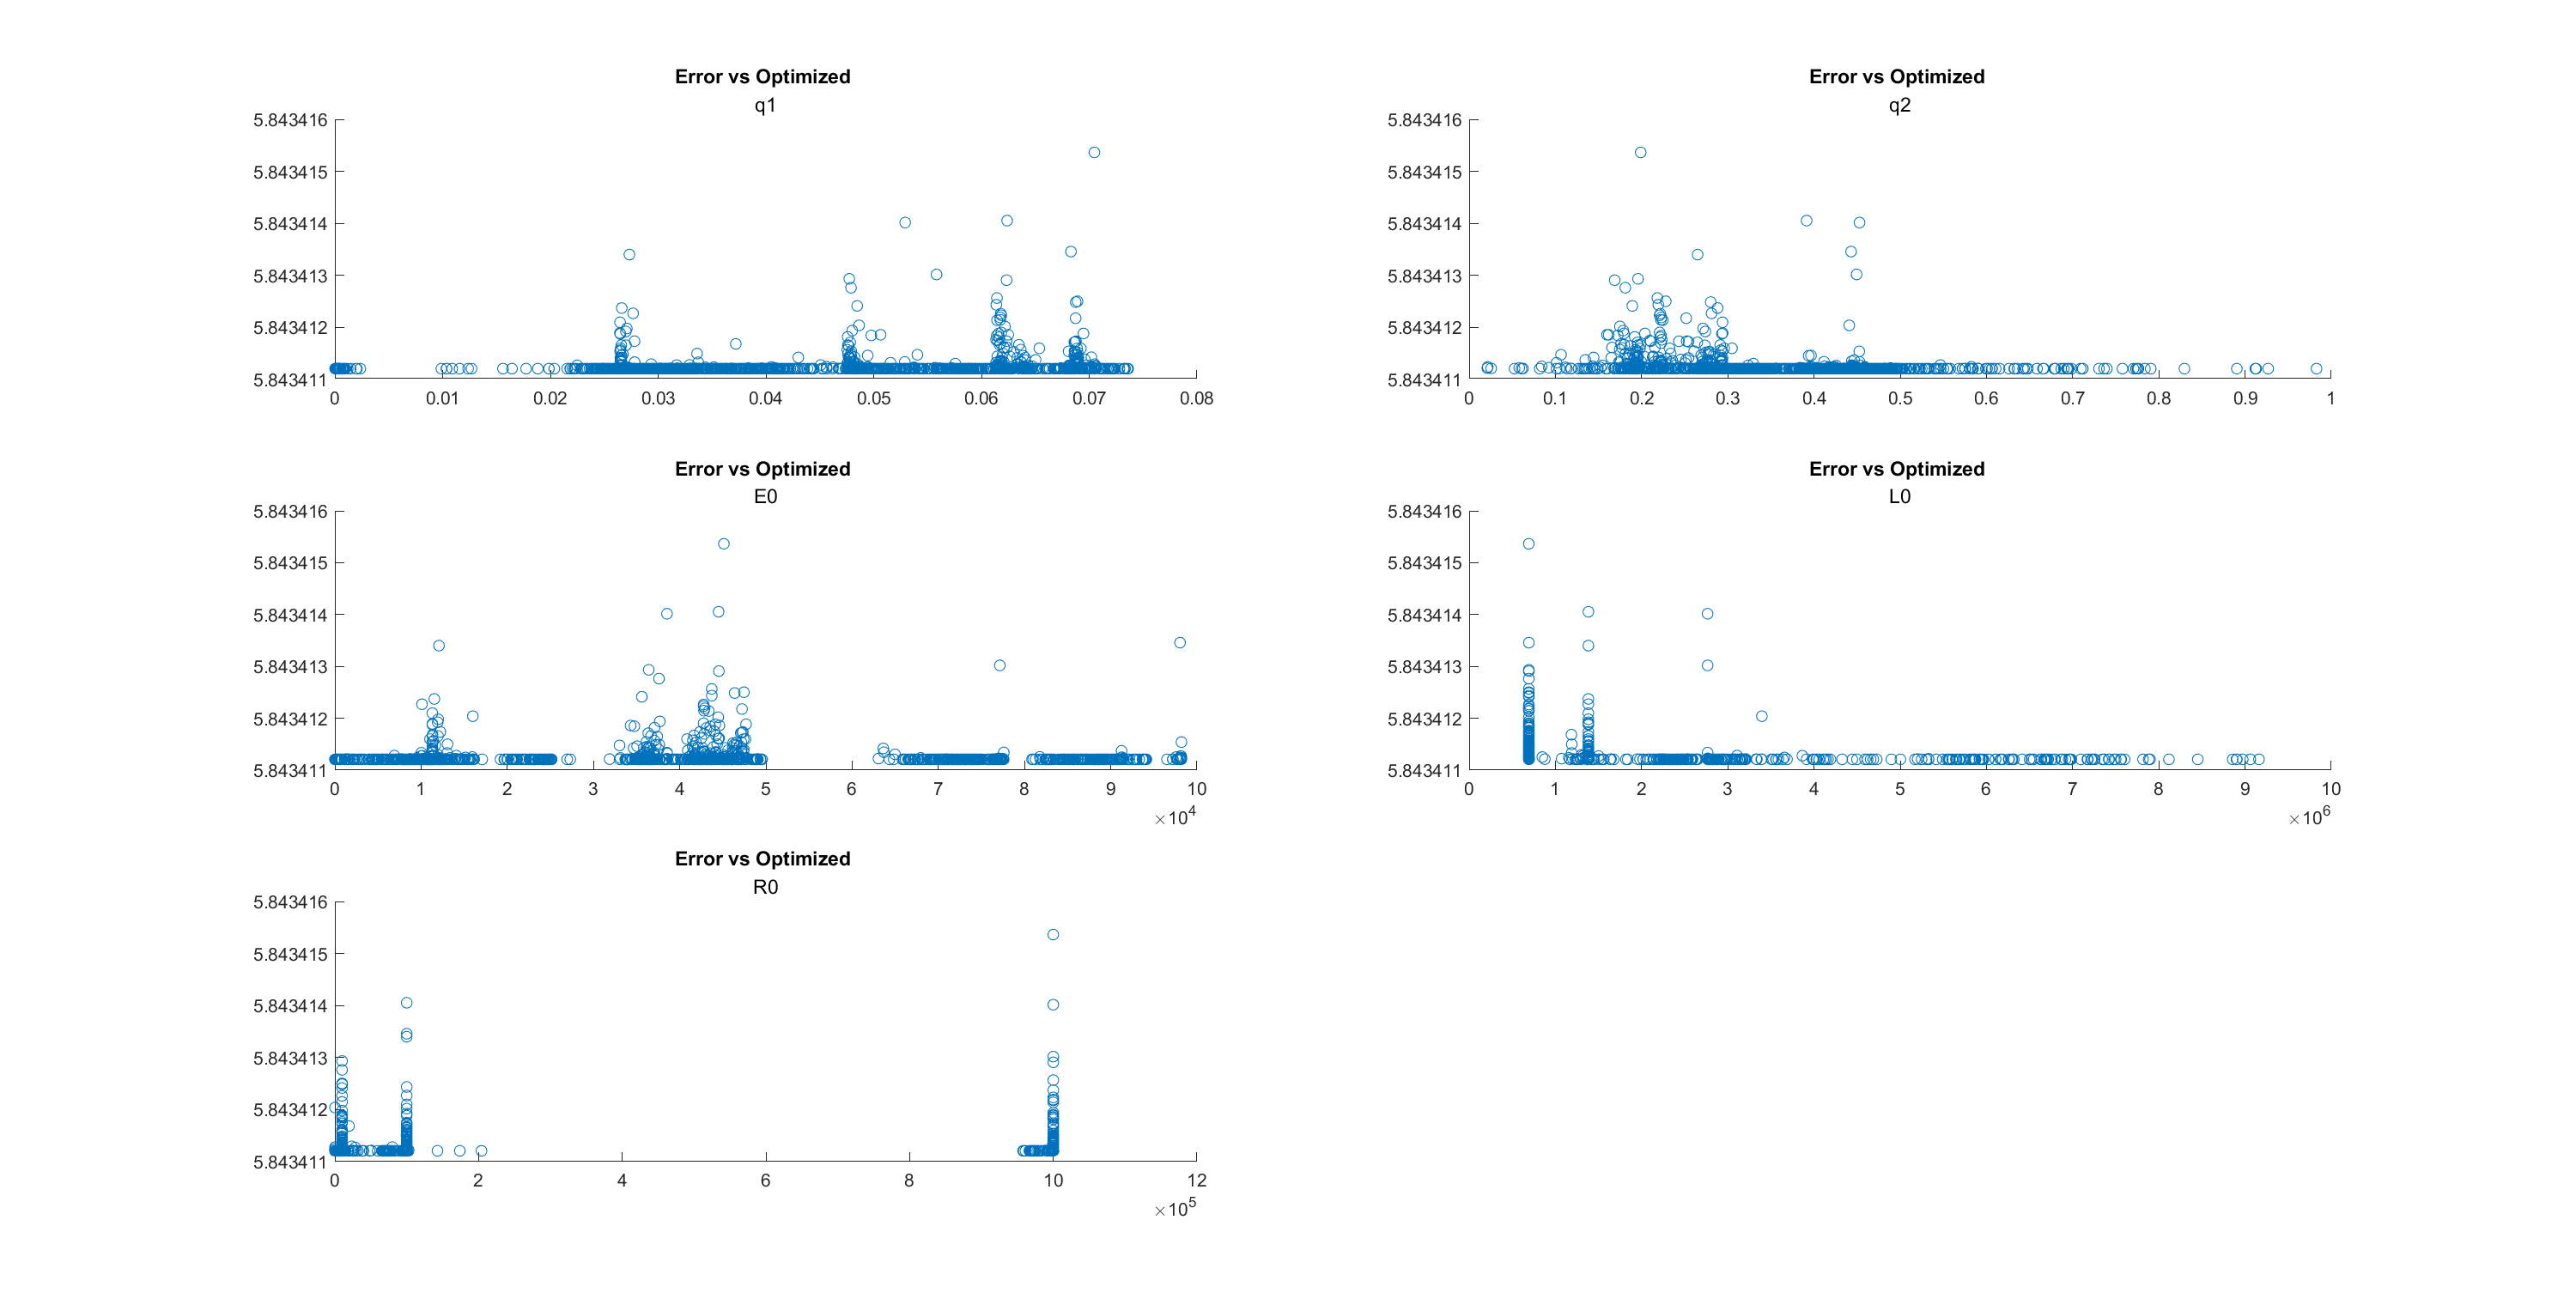
\includegraphics[width=0.8\textwidth]{ScatterPlotErrorVsOptimalOutput_Cut3.png}
	
	\caption{Scatter plot of the error vs optimized parameter. As we zoom in and delete outliers, we see more apparent outliers.  Will Ruth: ``This is what the tail of a distribution will often look like. It suggests that the outliers aren't typos".}
	
	\label{fig:ScatterErrorVsOptimizedParam}
\end{figure}


\section{Steady state as initial condition}

To address issue (2), which highlights the need for accurate initial specifications for $L_0$ and $R_0$, instead of using the initial conditions from \cite{GuoWu}, we simulate to steady states, and use the steady state as the initial condition.

\subsection{Pointwise stationary approximation}

In queuing theory, the pointwise stationary approximation of a queue system approximates any time of a queue system using its steady state (holding any time-dependent parameters constant) \cite{Green1991ThePS}.

Borrowing this idea, we estimate the initial conditions using the steady state of the system of DEs, which has a globally asymptotically stable unique endemic equilibrium \cite{GuoWu}.  We fix the time-dependent parameter immigration rate $\pi$ at reported value in 2010, then numerically simulate to steady state.  We have three ways to assess the accuracy of this approximation:
\begin{enumerate}
	\item Compare the steady state's total population to the reported total population.
	\item Compare the steady state's $T_0$, which is reported to be 1054.
	\item Compare the steady state's estimated incidence, which is reported to be 14.1.
\end{enumerate}

By these metrics, the steady state does reasonably well; see figure \ref{fig:PopVsTime_Various}.  This suggests the steady state can be used, either to help specify the initial condition, or to remove variables from the set of inputs.



\begin{figure}
		\centering
	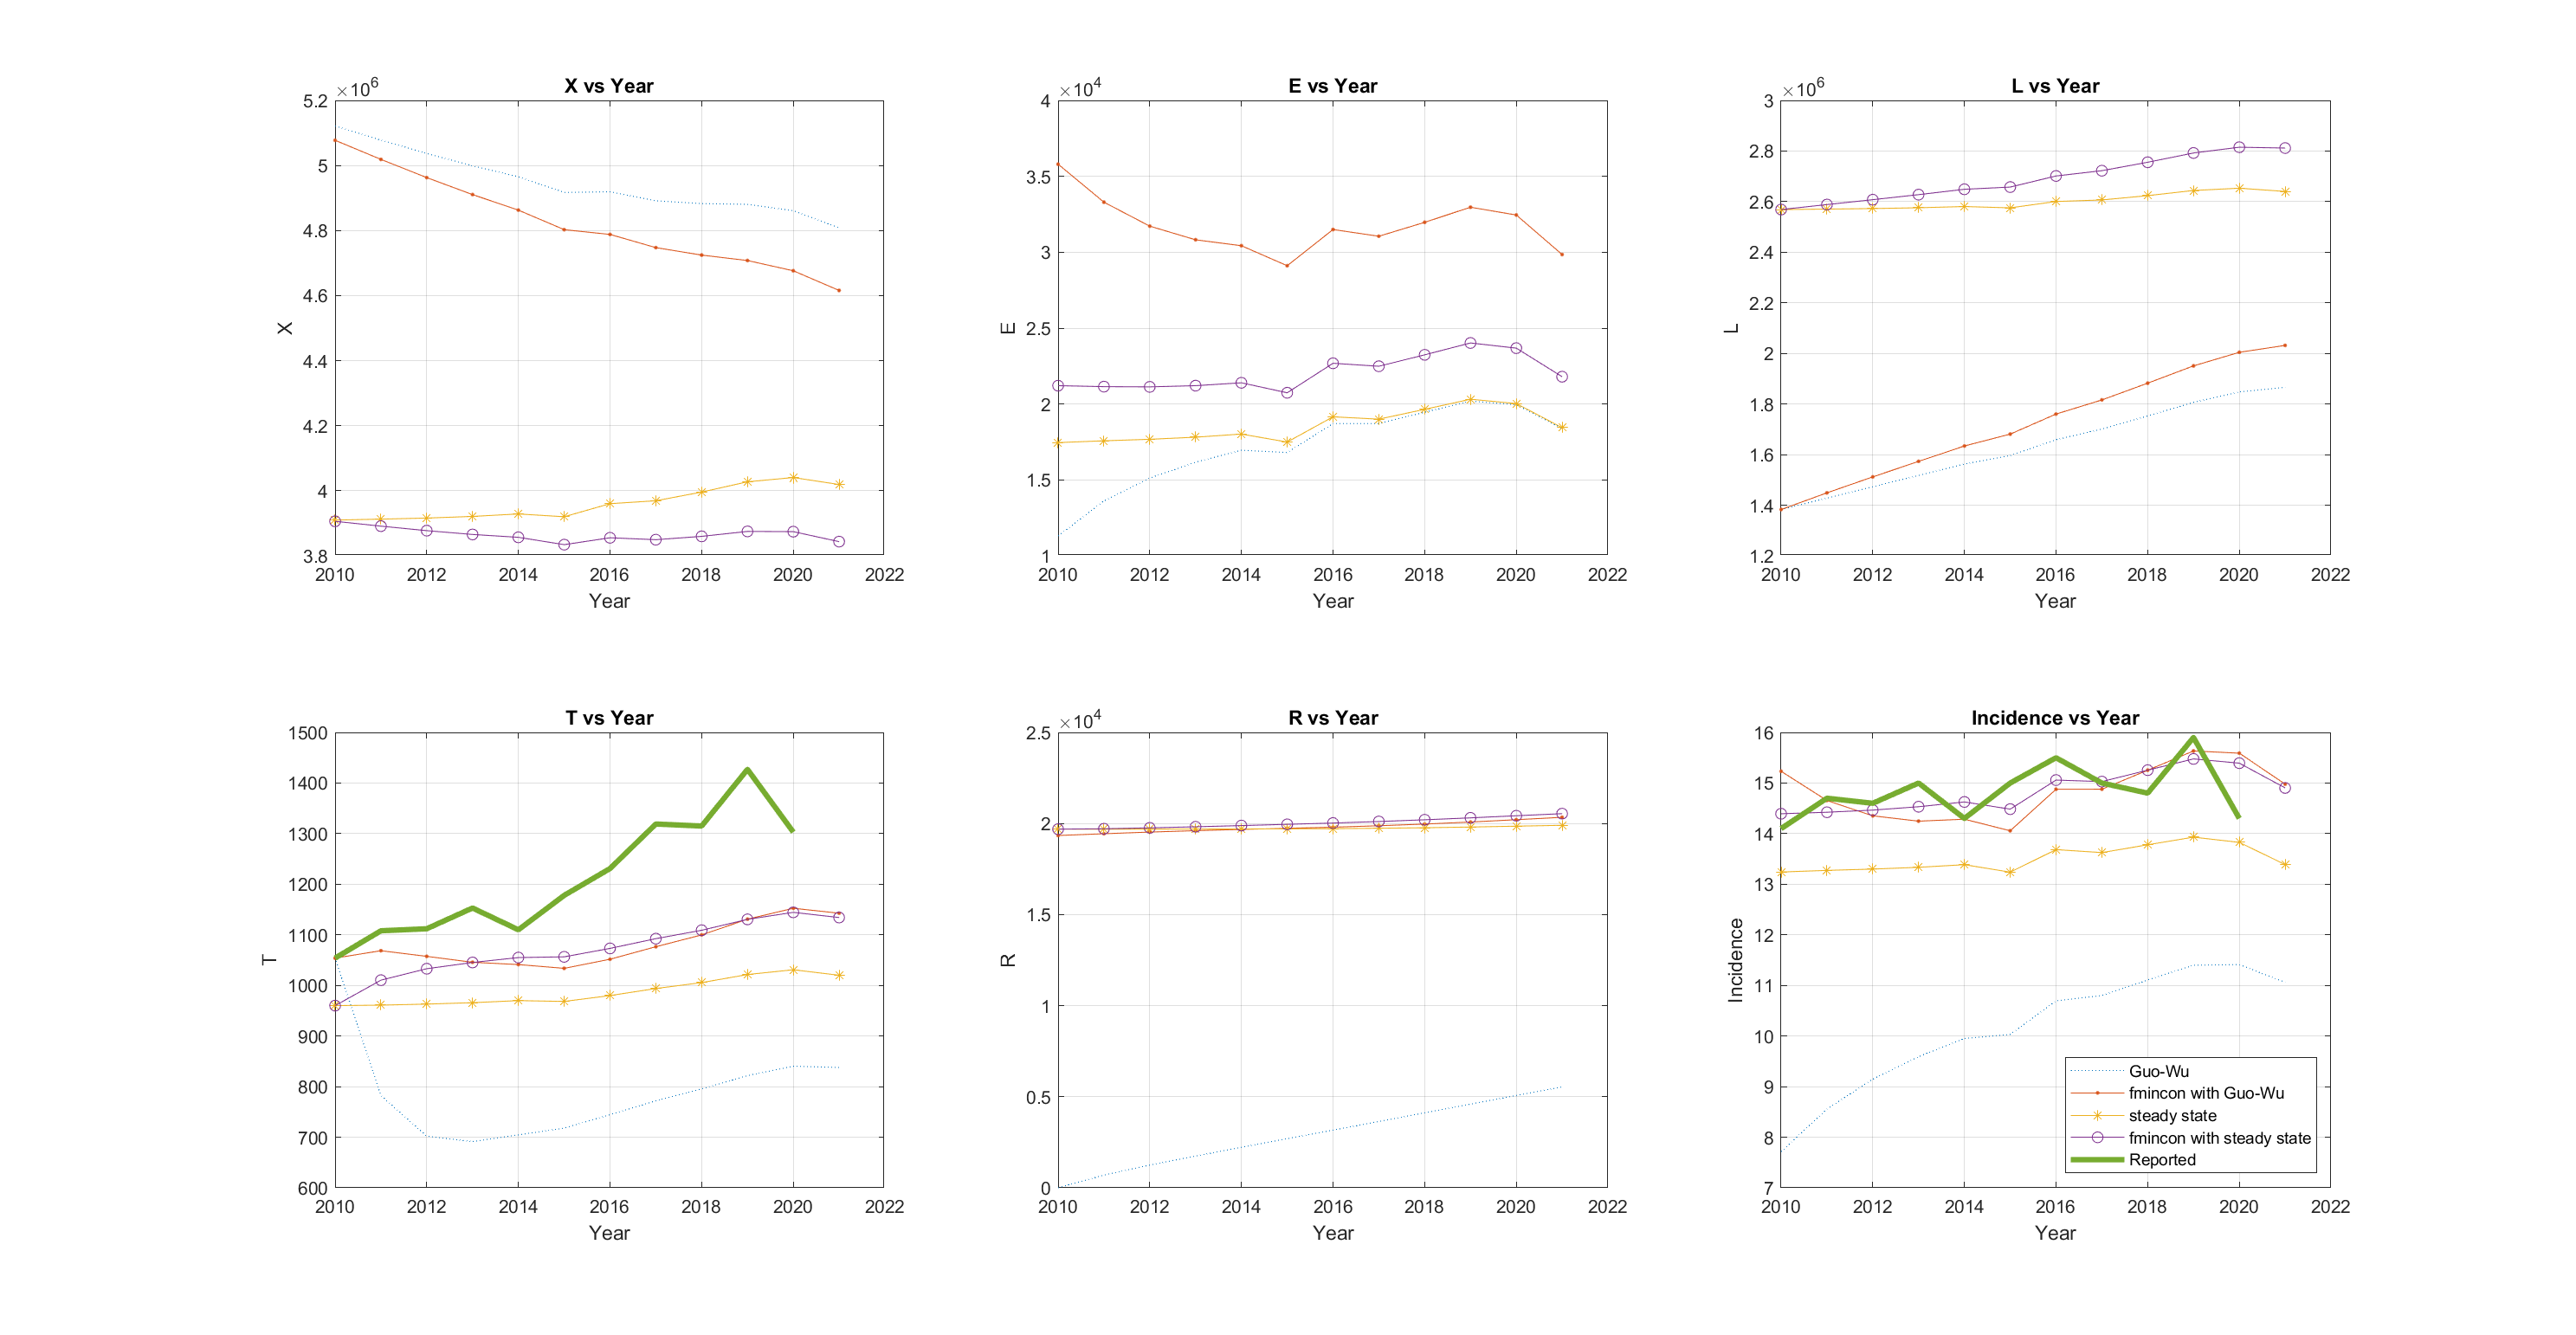
\includegraphics[width=\textwidth]{PopVsTime_various} 
	
	\caption{Even without optimization, the steady state is quite close to the reported incidence and prevalence.}
	
	\label{fig:PopVsTime_Various}
\end{figure}



\subsection{Sensitivity analysis on $L_0$ and $R_0$}

To study the effects of using steady states as initial conditions, we perform sensitivity analysis across various values of $E_0$, $L_0$, and $R_0$.  Sensitive parameters ($\nu$ and $\omega$) are held constant so we can ignore their effects for now.  Figure \ref{fig:HistoOptimalSS} shows our optimizer is no longer sensitive to the initial condition of $L_0$ and $R_0$, which is good.
	


	Earlier, our solver had issues with the initial conditions of $L_0$ and $R_0$.  Now, our results are most sensitive to $q_1$ and $q_2$, suggesting we are ready to pick realistic values of $q_1$ and $q_2$ to proceed.
	\begin{figure}
	\centering
			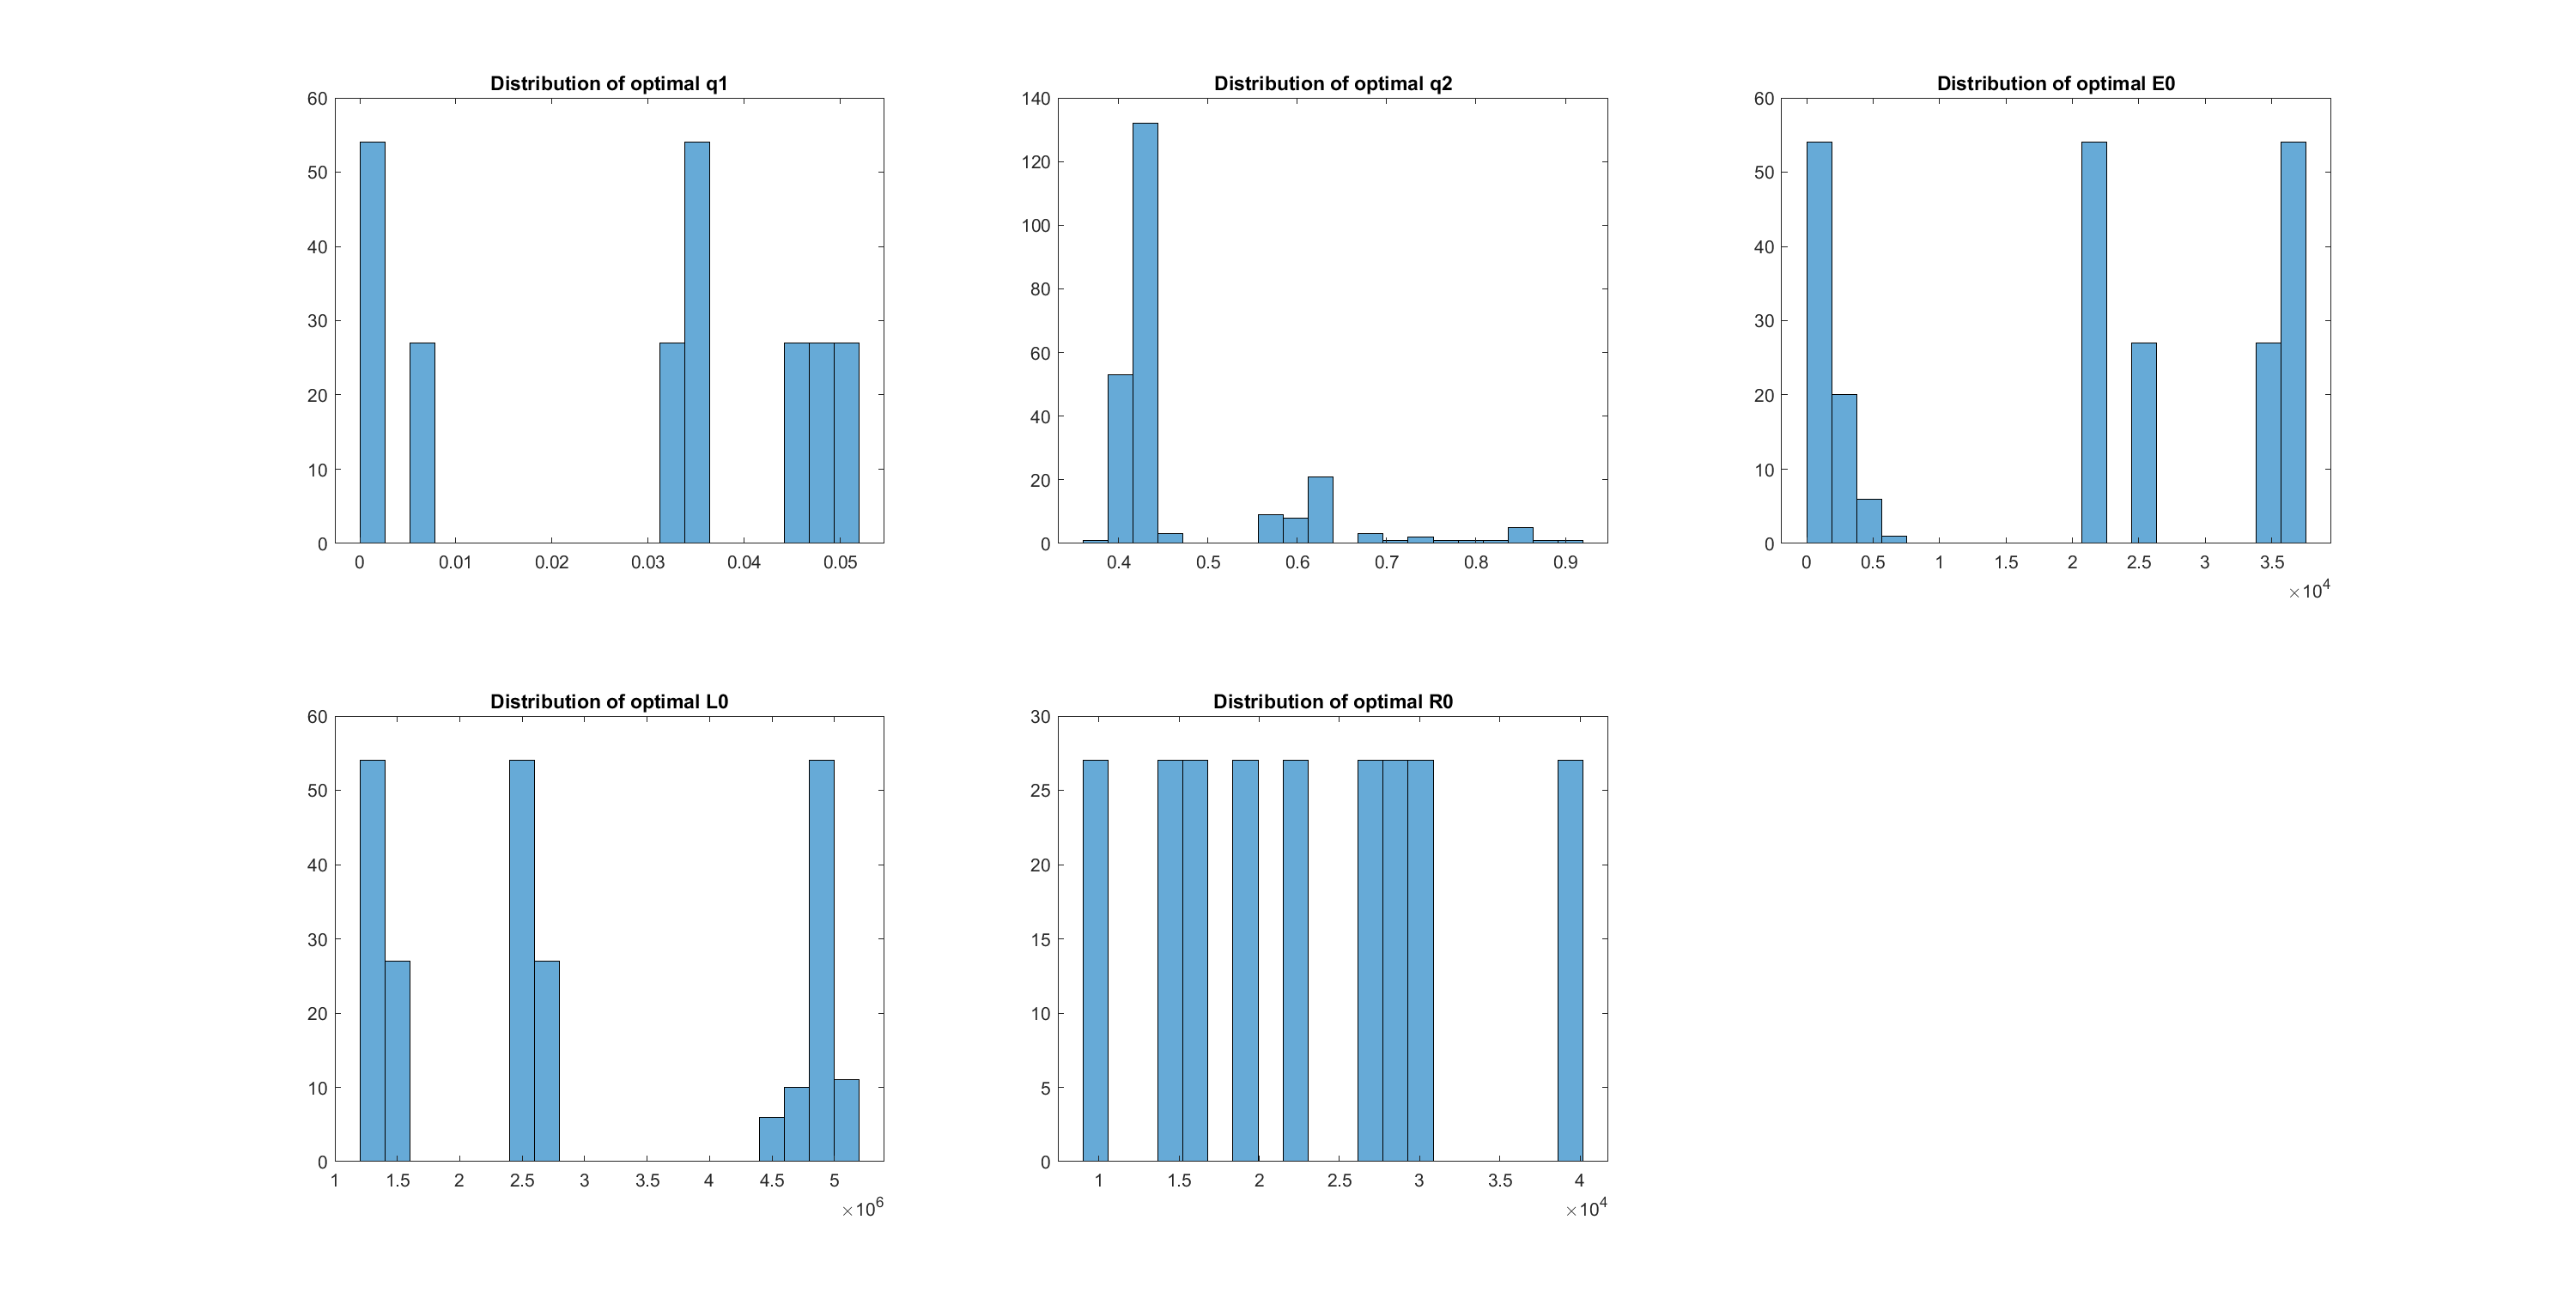
\includegraphics[width=0.45\textwidth]{Optimized parameter distribution across sensitivity analysis run4.png}  ~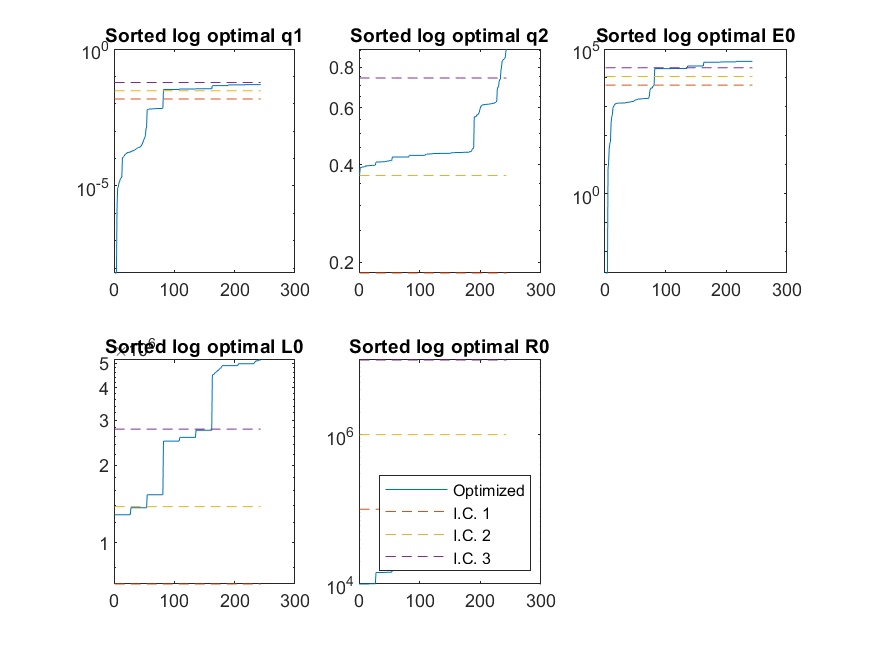
\includegraphics[width=0.45\textwidth]{Optimized parameter log sorted with starting values run4.png}
			\vskip\baselineskip
	
	\begin{subfigure}[b]{0.475\textwidth}
		\centering
		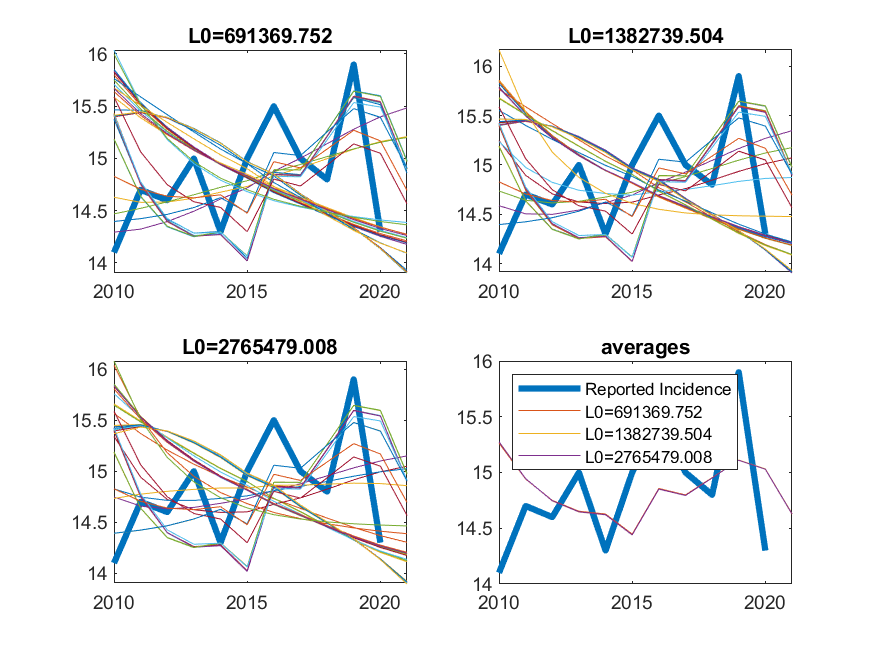
\includegraphics[width=\textwidth]{Sensitivty_L0 run4.png}
	\end{subfigure} 
	\hfill   
	\begin{subfigure}[b]{0.475\textwidth}
		\centering
		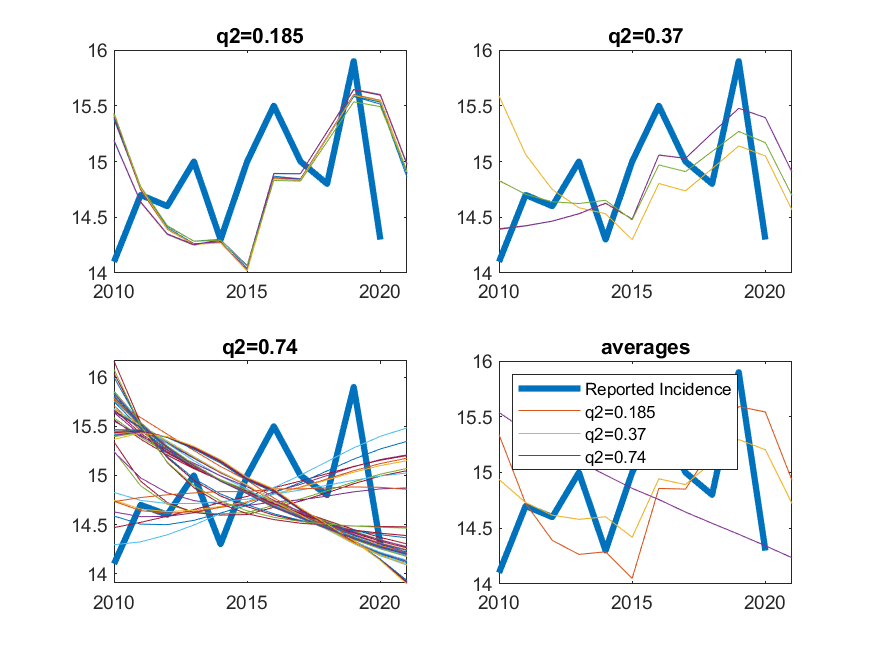
\includegraphics[width=\textwidth]{Sensitivty_q2 run4.png}  
	\end{subfigure} 
	
	\caption{After updating initial conditions to be steady states, the optimal results were not dependent on $L_0$ or $R_0$.  Instead, the response was most sensitive to $q_1$ and $q_2$.  We held $\nu$ and $\omega$ constant.}
	\label{fig:HistoOptimalSS}
\end{figure}

\subsection{Sensitivity analysis on $\omega$, $\nu$, $q_1$, and $q_2$}

From earlier investigations, we found our results were most sensitive to $\omega$, $\nu$, $q_1$, and $q_2$.  We picked an initial condition for them, then scaled them by $(0.90).^{[1,0,-1,-2]},$ giving a total of $ 4^4 = 256$ combinations.  See figure \ref{fig:SensitivtyAverages5}, which shows the results are not sensitive to $\omega$, but somewhat sensitive to $\nu$, $q_1$, and $q_2$.  I suspect $\nu$ is the most important because $q_1$ and $q_2$ are thrown into the optimizer anyway.


	\begin{figure}
	\centering
	\begin{subfigure}[b]{0.475\textwidth}
		\centering
		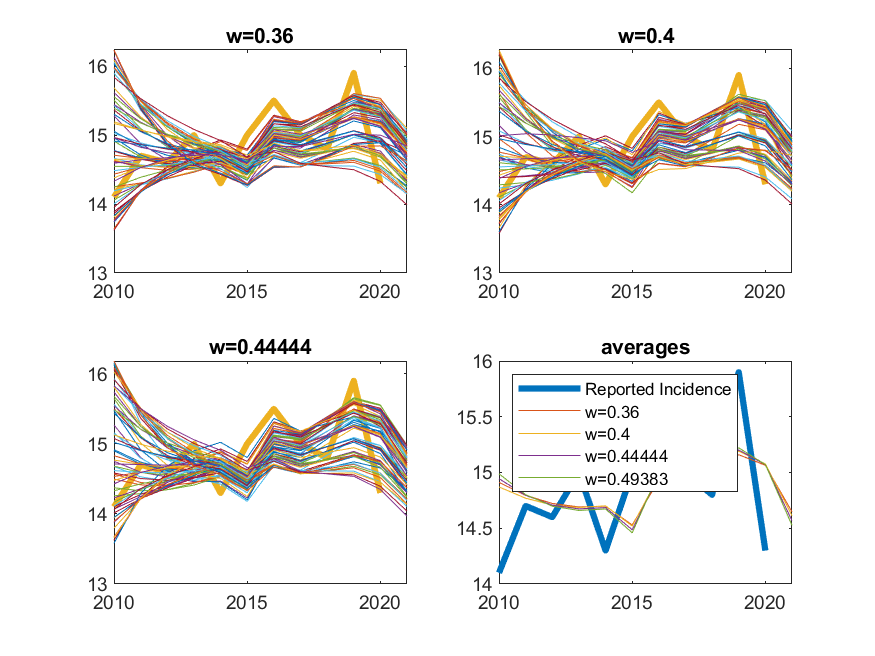
\includegraphics[width=\textwidth]{Sensitivty_wRun5.png}
	\end{subfigure} 
	\hfill   
	\begin{subfigure}[b]{0.475\textwidth}
		\centering
		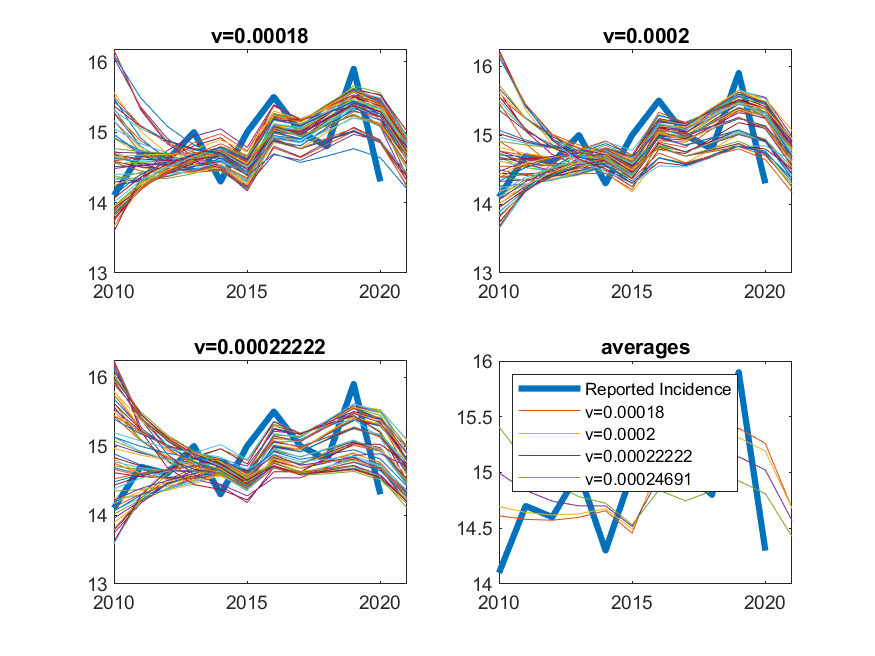
\includegraphics[width=\textwidth]{Sensitivty_vRun5.png}  
	\end{subfigure} 
	\vskip\baselineskip
	
	\begin{subfigure}[b]{0.475\textwidth}
		\centering
		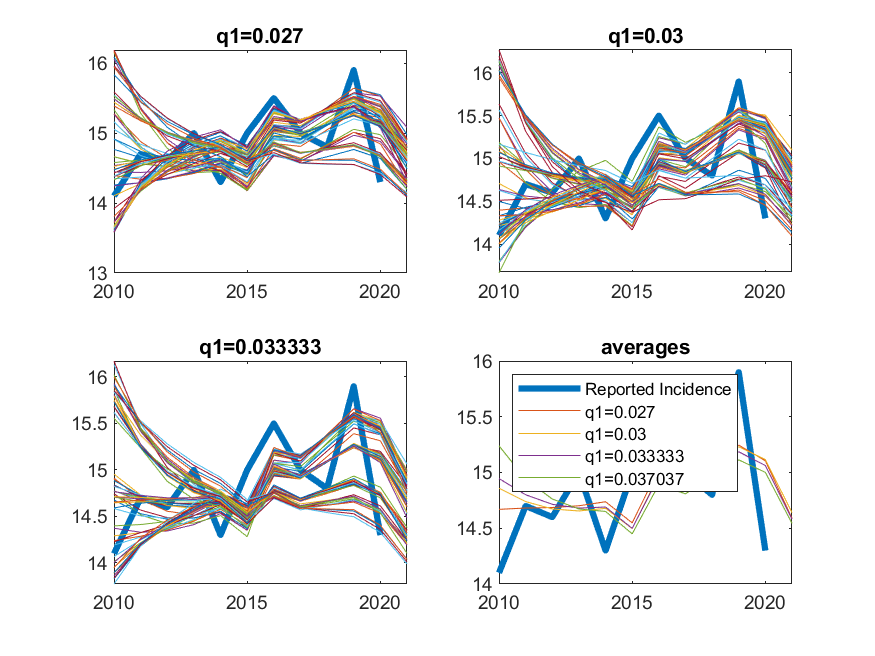
\includegraphics[width=\textwidth]{Sensitivty_q1Run5.png}  
	\end{subfigure} 
	\hfill
	\begin{subfigure}[b]{0.475\textwidth}
		\centering
		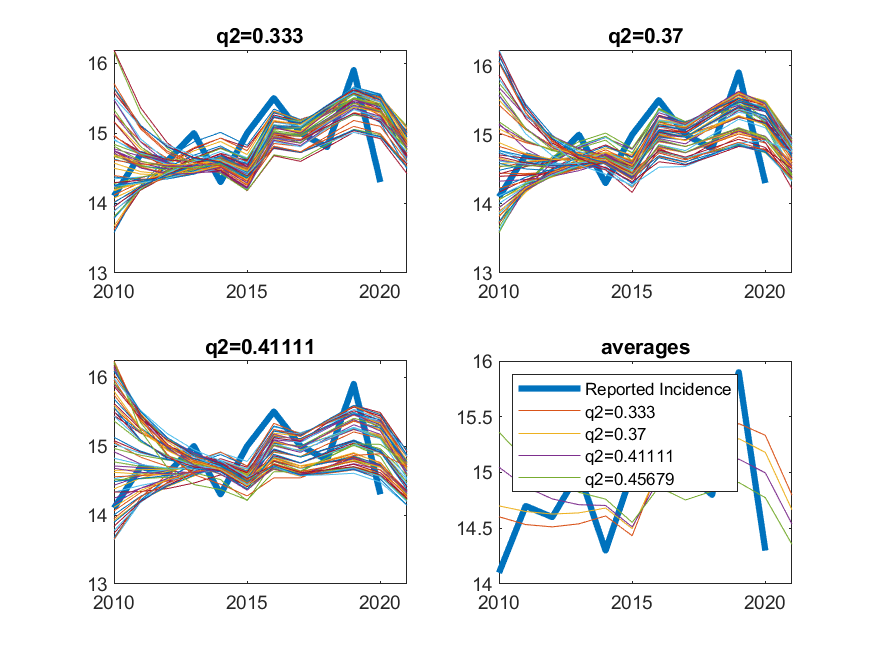
\includegraphics[width=\textwidth]{Sensitivty_q2Run5.png}  
	\end{subfigure} 
	
	\caption{I don't see anything irregular with these results.  The only things I notice is that as $\nu$ gets smaller, the incidence in 2010 improves.}
	\label{fig:SensitivtyAverages5}
\end{figure}

Figure \ref{fig:Histo5} shows the histogram of the optimal parameters.  $L_0$ is trimodal.  Otherwise, the other distributions look reasonably smooth.

\begin{figure}
	\centering
	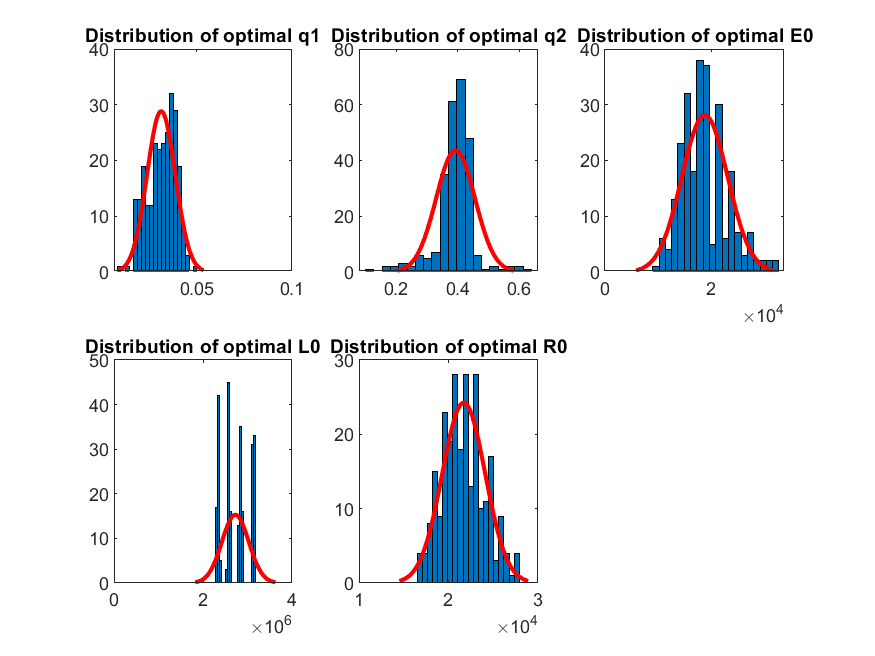
\includegraphics[scale=0.6]{Optimized parameter distribution across sensitivity analysisRun5}
	
	\caption{The most alarming histogram is the tri-modal $L_0$.  Only one initial condition for $L_0$ was specified.}
	
	\label{fig:Histo5}
\end{figure}

\subsection{Examining \texttt{fmincon} output}

Among the 256 experiments we performed during sensitivity analysis, we look at the set of parameters that minimize and maximize the errors, then examine some of $\texttt{fmincon}$'s outputs.  For the minimizing set, \texttt{fmincon} took 11 iterations with a total function count of 142.  This number is consistent with the fact that \texttt{fmincon} uses central finite differencing; since there are 5 dimensions, each gradient would cost 10 function evaluations (i.e. 110 function evaluations to evaluate the gradient).  Other factors like backtracking could contribute to the remaining 32 evaluations.
%, such as the gradient $\nabla f$ and hessian $H$.

\subsubsection{Gradient and Hessian}

We found
$$ \nabla f _{\text{min}} = [4.46e-03,~-1.56e-05,~-3.13e-10,~-7.99e-12,~2.76e-12 ] ,$$ 
and
$$ \nabla f _{\text{max}} = [4.09e-01,~-5.00e-03,~-1.21e-03,~-9.43e-06,~1.35e-09 ] .$$ 
Notice the largest partial derivatives are $f_{q_1}$ and $f_{q_2}$, while $f_{E_0}$, $f_{L_0}$, and $f_{R_0}$ are small.  This is consistent with our sensitivity analysis demonstrating that our model was most sensitive to $q_1$ and $q_2$.

Recall that we expect the gradient to approach zero near a minimum.  Notice that $$\| \nabla f_{\min} \|_\infty = 4.46 e-03 \ll \| \nabla f_{\max} \|_\infty = 4.09 e-01. $$  
$\nabla f_{\max}$ is 100 times larger than $ \nabla f_{\min} $, suggesting the the optimizer should continue searching at the maximum.  It turns out the error-maximizing parameter is poorly conditioned, which is demonstrated by the Hessian $H$.

Recall at a local minimum, the Hessian should be symmetric positive definite.  This is numerically verified by computing the eigenvalues of the Hessian matrix.  We found the eigenvalues $\lambda$
$$ \lambda(H_{\min})  = [5.2868e-04,~ 3.2415e-01,~1.0000e+00,~1.0000e+00,~8.4916e+05],$$ 
while
$$ \lambda(H_{\max})  =   [ 2.9168e-09,~1.0000e+00,~1.0000e+00,~1.5888e+02,~1.7682e+08].$$
Although all eigenvalues are positive, the small eigenvalues in $H_{\max}$ are driving the condition number up, which may be causing problems for the optimizer and thus the large gradient.
%So we again do sensitivity analysis



%Moreover, $\texttt{fmincon}$ uses the interior-point method to satisfy the constraints.  The Lagrange multipliers can be 


%	In addition to the above trajectory plots, we also investigate the distribution of parameter estimates across all configurations of the non-estimated parameters. Figure \ref{fig:est_dist} gives a histogram for our final estimates of each of $q_1$, $q_2$, $E_0$, $L_0$ and $R_0$. These histograms display the range of values for each parameter. Recall that $\cL_0$ is minimally affected by optimization, so the three bars in its histogram correspond to the three initial values for this parameter. \hl{Is next sentence a typo?} 
	

	
	
	
	
	\section{Future work and other attempts}
	
\begin{enumerate}
		\item \emph{Global optimization toolbox}.  I coded \texttt{multistart}, but found the solutions were still sensitive to the initial conditions we specified. 
	\item From figure \ref{fig:foreignBornData}, we see that immigration rate drives incidence.  Currently our initial condition is set in 2010, but perhaps it should be in 2009 instead (i.e., a year before the data set).  The immigration rate $\pi(2009)$ would likely be helpful.
	\item Investigate the multi-modal nature of $L_0$.
	\item Newly infected patients ($\leq2$ years from infection) are $15\times$ more likely to develop active TB than people with no known risk factor \cite{PublicHealthAgencyofCanada2014CanadianStandards}, hence $$ p\omega = 15 \cdot \nu . $$  This can be compared to our choices of $\omega$ and $\nu$.
	
	
	\item Will's suggestion:  Aim to reduce variability among optimal $q_1$ and $E_0$.  Among all the optimal $q_1$, we can measure variability by computing standard deviation divided by its mean. 

		\item Estimate derivative analytically.  Computing partial derivatives gets complicated because the loss function involves an integral of a high-dimensional function.  The main benefit, according to Sandy and JF, was savings in computational time (\texttt{fmincon} uses finite differencing to estimate derivative), but otherwise would not help our optimizer much.
		
\item Find upper bound by looking at actual immigration data.  We've currently collected a breakdown of which countries Canadian immigrants arrived from for the years 2016-2020 and are continuing to expand this collection.  Afterward, we could bucket countries into high-incidence and low-incidence, which can help improve estimates our of $q_1$ and $q_2$.
	
\end{enumerate}



\bibliographystyle{plain} % We choose the "plain" reference style
\bibliography{tb-bib}


\end{document}
